\documentclass[1p]{elsarticle_modified}
%\bibliographystyle{elsarticle-num}

%\usepackage[colorlinks]{hyperref}
%\usepackage{abbrmath_seonhwa} %\Abb, \Ascr, \Acal ,\Abf, \Afrak
\usepackage{amsfonts}
\usepackage{amssymb}
\usepackage{amsmath}
\usepackage{amsthm}
\usepackage{scalefnt}
\usepackage{amsbsy}
\usepackage{kotex}
\usepackage{caption}
\usepackage{subfig}
\usepackage{color}
\usepackage{graphicx}
\usepackage{xcolor} %% white, black, red, green, blue, cyan, magenta, yellow
\usepackage{float}
\usepackage{setspace}
\usepackage{hyperref}

\usepackage{tikz}
\usetikzlibrary{arrows}

\usepackage{multirow}
\usepackage{array} % fixed length table
\usepackage{hhline}

%%%%%%%%%%%%%%%%%%%%%
\makeatletter
\renewcommand*\env@matrix[1][\arraystretch]{%
	\edef\arraystretch{#1}%
	\hskip -\arraycolsep
	\let\@ifnextchar\new@ifnextchar
	\array{*\c@MaxMatrixCols c}}
\makeatother %https://tex.stackexchange.com/questions/14071/how-can-i-increase-the-line-spacing-in-a-matrix
%%%%%%%%%%%%%%%

\usepackage[normalem]{ulem}

\newcommand{\msout}[1]{\ifmmode\text{\sout{\ensuremath{#1}}}\else\sout{#1}\fi}
%SOURCE: \msout is \stkout macro in https://tex.stackexchange.com/questions/20609/strikeout-in-math-mode

\newcommand{\cancel}[1]{
	\ifmmode
	{\color{red}\msout{#1}}
	\else
	{\color{red}\sout{#1}}
	\fi
}

\newcommand{\add}[1]{
	{\color{blue}\uwave{#1}}
}

\newcommand{\replace}[2]{
	\ifmmode
	{\color{red}\msout{#1}}{\color{blue}\uwave{#2}}
	\else
	{\color{red}\sout{#1}}{\color{blue}\uwave{#2}}
	\fi
}

\newcommand{\Sol}{\mathcal{S}} %segment
\newcommand{\D}{D} %diagram
\newcommand{\A}{\mathcal{A}} %arc


%%%%%%%%%%%%%%%%%%%%%%%%%%%%%5 test

\def\sl{\operatorname{\textup{SL}}(2,\Cbb)}
\def\psl{\operatorname{\textup{PSL}}(2,\Cbb)}
\def\quan{\mkern 1mu \triangleright \mkern 1mu}

\theoremstyle{definition}
\newtheorem{thm}{Theorem}[section]
\newtheorem{prop}[thm]{Proposition}
\newtheorem{lem}[thm]{Lemma}
\newtheorem{ques}[thm]{Question}
\newtheorem{cor}[thm]{Corollary}
\newtheorem{defn}[thm]{Definition}
\newtheorem{exam}[thm]{Example}
\newtheorem{rmk}[thm]{Remark}
\newtheorem{alg}[thm]{Algorithm}

\newcommand{\I}{\sqrt{-1}}
\begin{document}

%\begin{frontmatter}
%
%\title{Boundary parabolic representations of knots up to 8 crossings}
%
%%% Group authors per affiliation:
%\author{Yunhi Cho} 
%\address{Department of Mathematics, University of Seoul, Seoul, Korea}
%\ead{yhcho@uos.ac.kr}
%
%
%\author{Seonhwa Kim} %\fnref{s_kim}}
%\address{Center for Geometry and Physics, Institute for Basic Science, Pohang, 37673, Korea}
%\ead{ryeona17@ibs.re.kr}
%
%\author{Hyuk Kim}
%\address{Department of Mathematical Sciences, Seoul National University, Seoul 08826, Korea}
%\ead{hyukkim@snu.ac.kr}
%
%\author{Seokbeom Yoon}
%\address{Department of Mathematical Sciences, Seoul National University, Seoul, 08826,  Korea}
%\ead{sbyoon15@snu.ac.kr}
%
%\begin{abstract}
%We find all boundary parabolic representation of knots up to 8 crossings.
%
%\end{abstract}
%\begin{keyword}
%    \MSC[2010] 57M25 
%\end{keyword}
%
%\end{frontmatter}

%\linenumbers
%\tableofcontents
%
\newcommand\colored[1]{\textcolor{white}{\rule[-0.35ex]{0.8em}{1.4ex}}\kern-0.8em\color{red} #1}%
%\newcommand\colored[1]{\textcolor{white}{ #1}\kern-2.17ex	\textcolor{white}{ #1}\kern-1.81ex	\textcolor{white}{ #1}\kern-2.15ex\color{red}#1	}

{\Large $\underline{11a_{141}~(K11a_{141})}$}

\setlength{\tabcolsep}{10pt}
\renewcommand{\arraystretch}{1.6}
\vspace{1cm}\begin{tabular}{m{100pt}>{\centering\arraybackslash}m{274pt}}
\multirow{5}{120pt}{
	\centering
	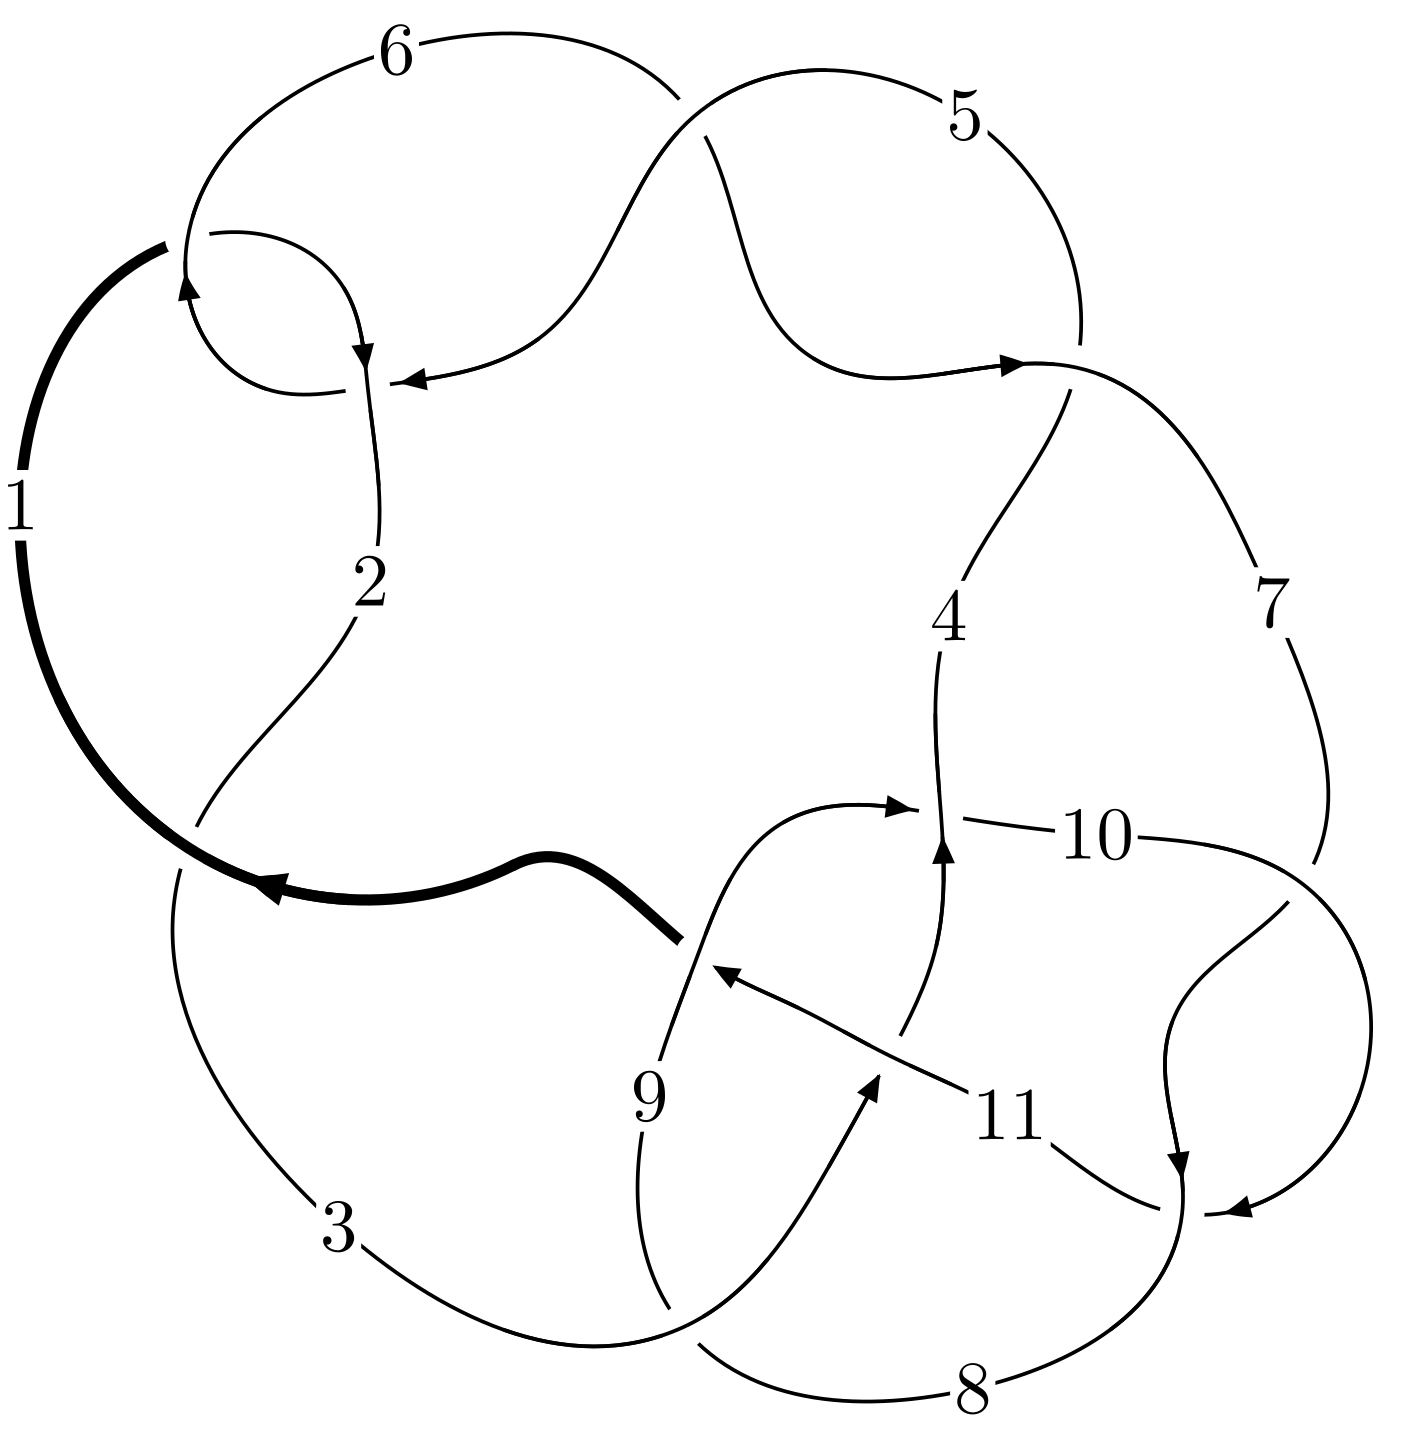
\includegraphics[width=112pt]{../../../GIT/diagram.site/Diagrams/png/390_11a_141.png}\\
\ \ \ A knot diagram\footnotemark}&
\allowdisplaybreaks
\textbf{Linearized knot diagam} \\
\cline{2-2}
 &
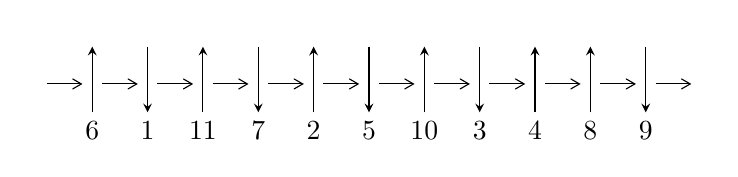
\begin{tikzpicture}[x=20pt, y=17pt]
	% nodes
	\node (C0) at (0, 0) {};
	\node (C1) at (1, 0) {};
	\node (C1U) at (1, +1) {};
	\node (C1D) at (1, -1) {6};

	\node (C2) at (2, 0) {};
	\node (C2U) at (2, +1) {};
	\node (C2D) at (2, -1) {1};

	\node (C3) at (3, 0) {};
	\node (C3U) at (3, +1) {};
	\node (C3D) at (3, -1) {11};

	\node (C4) at (4, 0) {};
	\node (C4U) at (4, +1) {};
	\node (C4D) at (4, -1) {7};

	\node (C5) at (5, 0) {};
	\node (C5U) at (5, +1) {};
	\node (C5D) at (5, -1) {2};

	\node (C6) at (6, 0) {};
	\node (C6U) at (6, +1) {};
	\node (C6D) at (6, -1) {5};

	\node (C7) at (7, 0) {};
	\node (C7U) at (7, +1) {};
	\node (C7D) at (7, -1) {10};

	\node (C8) at (8, 0) {};
	\node (C8U) at (8, +1) {};
	\node (C8D) at (8, -1) {3};

	\node (C9) at (9, 0) {};
	\node (C9U) at (9, +1) {};
	\node (C9D) at (9, -1) {4};

	\node (C10) at (10, 0) {};
	\node (C10U) at (10, +1) {};
	\node (C10D) at (10, -1) {8};

	\node (C11) at (11, 0) {};
	\node (C11U) at (11, +1) {};
	\node (C11D) at (11, -1) {9};
	\node (C12) at (12, 0) {};

	% arrows
	\draw[->,>={angle 60}]
	(C0) edge (C1) (C1) edge (C2) (C2) edge (C3) (C3) edge (C4) (C4) edge (C5) (C5) edge (C6) (C6) edge (C7) (C7) edge (C8) (C8) edge (C9) (C9) edge (C10) (C10) edge (C11) (C11) edge (C12) ;	\draw[->,>=stealth]
	(C1D) edge (C1U) (C2U) edge (C2D) (C3D) edge (C3U) (C4U) edge (C4D) (C5D) edge (C5U) (C6U) edge (C6D) (C7D) edge (C7U) (C8U) edge (C8D) (C9D) edge (C9U) (C10D) edge (C10U) (C11U) edge (C11D) ;
	\end{tikzpicture} \\
\hhline{~~} \\& 
\textbf{Solving Sequence} \\ \cline{2-2} 
 &
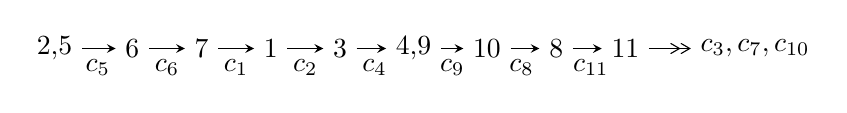
\begin{tikzpicture}[x=25pt, y=7pt]
	% node
	\node (A0) at (-1/8, 0) {2,5};
	\node (A1) at (1, 0) {6};
	\node (A2) at (2, 0) {7};
	\node (A3) at (3, 0) {1};
	\node (A4) at (4, 0) {3};
	\node (A5) at (81/16, 0) {4,9};
	\node (A6) at (49/8, 0) {10};
	\node (A7) at (57/8, 0) {8};
	\node (A8) at (65/8, 0) {11};
	\node (C1) at (1/2, -1) {$c_{5}$};
	\node (C2) at (3/2, -1) {$c_{6}$};
	\node (C3) at (5/2, -1) {$c_{1}$};
	\node (C4) at (7/2, -1) {$c_{2}$};
	\node (C5) at (9/2, -1) {$c_{4}$};
	\node (C6) at (45/8, -1) {$c_{9}$};
	\node (C7) at (53/8, -1) {$c_{8}$};
	\node (C8) at (61/8, -1) {$c_{11}$};
	\node (A9) at (10, 0) {$c_{3},c_{7},c_{10}$};

	% edge
	\draw[->,>=stealth]	
	(A0) edge (A1) (A1) edge (A2) (A2) edge (A3) (A3) edge (A4) (A4) edge (A5) (A5) edge (A6) (A6) edge (A7) (A7) edge (A8) ;
	\draw[->>,>={angle 60}]	
	(A8) edge (A9);
\end{tikzpicture} \\ 

\end{tabular} \\

\footnotetext{
The image of knot diagram is generated by the software ``\textbf{Draw programme}" developed by Andrew Bartholomew(\url{http://www.layer8.co.uk/maths/draw/index.htm\#Running-draw}), where we modified some parts for our purpose(\url{https://github.com/CATsTAILs/LinksPainter}).
}\phantom \\ \newline 
\centering \textbf{Ideals for irreducible components\footnotemark of $X_{\text{par}}$} 
 
\begin{align*}
I^u_{1}&=\langle 
4.26487\times10^{16} u^{52}-5.40372\times10^{16} u^{51}+\cdots+1.36187\times10^{16} b+1.03514\times10^{16},\\
\phantom{I^u_{1}}&\phantom{= \langle  }-5.55636\times10^{16} u^{52}-1.64714\times10^{16} u^{51}+\cdots+4.08560\times10^{16} a+3.29067\times10^{16},\;u^{53}-2 u^{52}+\cdots+5 u-1\rangle \\
I^u_{2}&=\langle 
b- u,\;a+1,\;u^2- u+1\rangle \\
\\
\end{align*}
\raggedright * 2 irreducible components of $\dim_{\mathbb{C}}=0$, with total 55 representations.\\
\footnotetext{All coefficients of polynomials are rational numbers. But the coefficients are sometimes approximated in decimal forms when there is not enough margin.}
\newpage
\renewcommand{\arraystretch}{1}
\centering \section*{I. $I^u_{1}= \langle 4.26\times10^{16} u^{52}-5.40\times10^{16} u^{51}+\cdots+1.36\times10^{16} b+1.04\times10^{16},\;-5.56\times10^{16} u^{52}-1.65\times10^{16} u^{51}+\cdots+4.09\times10^{16} a+3.29\times10^{16},\;u^{53}-2 u^{52}+\cdots+5 u-1 \rangle$}
\flushleft \textbf{(i) Arc colorings}\\
\begin{tabular}{m{7pt} m{180pt} m{7pt} m{180pt} }
\flushright $a_{2}=$&$\begin{pmatrix}0\\u\end{pmatrix}$ \\
\flushright $a_{5}=$&$\begin{pmatrix}1\\0\end{pmatrix}$ \\
\flushright $a_{6}=$&$\begin{pmatrix}1\\- u^2\end{pmatrix}$ \\
\flushright $a_{7}=$&$\begin{pmatrix}u^2+1\\- u^2\end{pmatrix}$ \\
\flushright $a_{1}=$&$\begin{pmatrix}- u\\u^3+u\end{pmatrix}$ \\
\flushright $a_{3}=$&$\begin{pmatrix}- u^3\\u^5+u^3+u\end{pmatrix}$ \\
\flushright $a_{4}=$&$\begin{pmatrix}u^4+u^2+1\\- u^4\end{pmatrix}$ \\
\flushright $a_{9}=$&$\begin{pmatrix}1.35999 u^{52}+0.403157 u^{51}+\cdots+12.2341 u-0.805431\\-3.13164 u^{52}+3.96788 u^{51}+\cdots+3.80587 u-0.760087\end{pmatrix}$ \\
\flushright $a_{10}=$&$\begin{pmatrix}-0.239857 u^{52}+2.87394 u^{51}+\cdots+17.1081 u-2.41707\\-3.38916 u^{52}+5.76021 u^{51}+\cdots+10.4571 u-2.36000\end{pmatrix}$ \\
\flushright $a_{8}=$&$\begin{pmatrix}-0.240103 u^{52}+2.73675 u^{51}+\cdots+17.6038 u-1.54783\\-3.25991 u^{52}+5.55889 u^{51}+\cdots+10.1878 u-2.35999\end{pmatrix}$ \\
\flushright $a_{11}=$&$\begin{pmatrix}0.200023 u^{52}+0.0418941 u^{51}+\cdots+1.97228 u+0.477613\\-0.441941 u^{52}-0.197074 u^{51}+\cdots+0.522504 u-0.200023\end{pmatrix}$\\ \flushright $a_{11}=$&$\begin{pmatrix}0.200023 u^{52}+0.0418941 u^{51}+\cdots+1.97228 u+0.477613\\-0.441941 u^{52}-0.197074 u^{51}+\cdots+0.522504 u-0.200023\end{pmatrix}$\\&\end{tabular}
\flushleft \textbf{(ii) Obstruction class $= -1$}\\~\\
\flushleft \textbf{(iii) Cusp Shapes $= -\frac{275359995103539017}{13618658791677283} u^{52}+\frac{577412524426465435}{13618658791677283} u^{51}+\cdots+\frac{1768558808672064537}{13618658791677283} u-\frac{316215934356851336}{13618658791677283}$}\\~\\
\newpage\renewcommand{\arraystretch}{1}
\flushleft \textbf{(iv) u-Polynomials at the component}\newline \\
\begin{tabular}{m{50pt}|m{274pt}}
Crossings & \hspace{64pt}u-Polynomials at each crossing \\
\hline $$\begin{aligned}c_{1},c_{5}\end{aligned}$$&$\begin{aligned}
&u^{53}-2 u^{52}+\cdots+5 u-1
\end{aligned}$\\
\hline $$\begin{aligned}c_{2},c_{4},c_{6}\end{aligned}$$&$\begin{aligned}
&u^{53}+12 u^{52}+\cdots+u-1
\end{aligned}$\\
\hline $$\begin{aligned}c_{3}\end{aligned}$$&$\begin{aligned}
&u^{53}+4 u^{52}+\cdots+u+1
\end{aligned}$\\
\hline $$\begin{aligned}c_{7},c_{10}\end{aligned}$$&$\begin{aligned}
&u^{53}+3 u^{52}+\cdots+8 u-1
\end{aligned}$\\
\hline $$\begin{aligned}c_{8}\end{aligned}$$&$\begin{aligned}
&u^{53}+2 u^{52}+\cdots+361 u-31
\end{aligned}$\\
\hline $$\begin{aligned}c_{9}\end{aligned}$$&$\begin{aligned}
&u^{53}+10 u^{51}+\cdots-4625 u-6737
\end{aligned}$\\
\hline $$\begin{aligned}c_{11}\end{aligned}$$&$\begin{aligned}
&u^{53}-9 u^{52}+\cdots-4 u-4
\end{aligned}$\\
\hline
\end{tabular}\\~\\
\newpage\renewcommand{\arraystretch}{1}
\flushleft \textbf{(v) Riley Polynomials at the component}\newline \\
\begin{tabular}{m{50pt}|m{274pt}}
Crossings & \hspace{64pt}Riley Polynomials at each crossing \\
\hline $$\begin{aligned}c_{1},c_{5}\end{aligned}$$&$\begin{aligned}
&y^{53}+12 y^{52}+\cdots+y-1
\end{aligned}$\\
\hline $$\begin{aligned}c_{2},c_{4},c_{6}\end{aligned}$$&$\begin{aligned}
&y^{53}+60 y^{52}+\cdots+185 y-1
\end{aligned}$\\
\hline $$\begin{aligned}c_{3}\end{aligned}$$&$\begin{aligned}
&y^{53}-8 y^{52}+\cdots+y-1
\end{aligned}$\\
\hline $$\begin{aligned}c_{7},c_{10}\end{aligned}$$&$\begin{aligned}
&y^{53}-43 y^{52}+\cdots-84 y-1
\end{aligned}$\\
\hline $$\begin{aligned}c_{8}\end{aligned}$$&$\begin{aligned}
&y^{53}+68 y^{52}+\cdots+28145 y-961
\end{aligned}$\\
\hline $$\begin{aligned}c_{9}\end{aligned}$$&$\begin{aligned}
&y^{53}+20 y^{52}+\cdots+623516737 y-45387169
\end{aligned}$\\
\hline $$\begin{aligned}c_{11}\end{aligned}$$&$\begin{aligned}
&y^{53}+15 y^{52}+\cdots-120 y-16
\end{aligned}$\\
\hline
\end{tabular}\\~\\
\newpage\flushleft \textbf{(vi) Complex Volumes and Cusp Shapes}
$$\begin{array}{c|c|c}  
\text{Solutions to }I^u_{1}& \I (\text{vol} + \sqrt{-1}CS) & \text{Cusp shape}\\
 \hline 
\begin{aligned}
u &= -0.441064 + 0.891798 I \\
a &= -1.020870 - 0.571634 I \\
b &= \phantom{-}0.328536 + 0.775979 I\end{aligned}
 & -0.83694 - 5.74776 I & \phantom{-0.000000 -}0. + 9.66844 I \\ \hline\begin{aligned}
u &= -0.441064 - 0.891798 I \\
a &= -1.020870 + 0.571634 I \\
b &= \phantom{-}0.328536 - 0.775979 I\end{aligned}
 & -0.83694 + 5.74776 I & \phantom{-0.000000 } 0. - 9.66844 I \\ \hline\begin{aligned}
u &= \phantom{-}0.049379 + 1.054040 I \\
a &= -0.0434698 + 0.0967864 I \\
b &= -0.695181 - 0.606165 I\end{aligned}
 & \phantom{-}0.26646 + 4.82522 I & \phantom{-}1.00000 - 6.65378 I \\ \hline\begin{aligned}
u &= \phantom{-}0.049379 - 1.054040 I \\
a &= -0.0434698 - 0.0967864 I \\
b &= -0.695181 + 0.606165 I\end{aligned}
 & \phantom{-}0.26646 - 4.82522 I & \phantom{-}1.00000 + 6.65378 I \\ \hline\begin{aligned}
u &= \phantom{-}0.648943 + 0.852337 I \\
a &= \phantom{-}0.538490 + 0.498386 I \\
b &= -0.203229 - 0.464579 I\end{aligned}
 & \phantom{-}0.64509 + 2.50411 I & -2.75636 - 4.40791 I \\ \hline\begin{aligned}
u &= \phantom{-}0.648943 - 0.852337 I \\
a &= \phantom{-}0.538490 - 0.498386 I \\
b &= -0.203229 + 0.464579 I\end{aligned}
 & \phantom{-}0.64509 - 2.50411 I & -2.75636 + 4.40791 I \\ \hline\begin{aligned}
u &= -0.499123 + 0.779146 I \\
a &= -1.020240 - 0.640877 I \\
b &= -0.424147 - 0.588184 I\end{aligned}
 & \phantom{-}3.37085 - 3.65736 I & \phantom{-}8.56973 + 8.26952 I \\ \hline\begin{aligned}
u &= -0.499123 - 0.779146 I \\
a &= -1.020240 + 0.640877 I \\
b &= -0.424147 + 0.588184 I\end{aligned}
 & \phantom{-}3.37085 + 3.65736 I & \phantom{-}8.56973 - 8.26952 I \\ \hline\begin{aligned}
u &= \phantom{-}0.360123 + 0.813464 I \\
a &= -0.143330 + 0.781657 I \\
b &= \phantom{-}0.328335 - 0.649856 I\end{aligned}
 & -0.31212 + 1.82370 I & -0.23465 - 3.74406 I \\ \hline\begin{aligned}
u &= \phantom{-}0.360123 - 0.813464 I \\
a &= -0.143330 - 0.781657 I \\
b &= \phantom{-}0.328335 + 0.649856 I\end{aligned}
 & -0.31212 - 1.82370 I & -0.23465 + 3.74406 I\\
 \hline 
 \end{array}$$\newpage$$\begin{array}{c|c|c}  
\text{Solutions to }I^u_{1}& \I (\text{vol} + \sqrt{-1}CS) & \text{Cusp shape}\\
 \hline 
\begin{aligned}
u &= -0.498548 + 1.006320 I \\
a &= \phantom{-}0.884968 + 0.778679 I \\
b &= -0.520382 - 0.426991 I\end{aligned}
 & \phantom{-}3.53599 - 10.89690 I & \phantom{-0.000000 -}0. + 9.33368 I \\ \hline\begin{aligned}
u &= -0.498548 - 1.006320 I \\
a &= \phantom{-}0.884968 - 0.778679 I \\
b &= -0.520382 + 0.426991 I\end{aligned}
 & \phantom{-}3.53599 + 10.89690 I & \phantom{-0.000000 } 0. - 9.33368 I \\ \hline\begin{aligned}
u &= -0.058697 + 0.871659 I \\
a &= -0.154861 + 0.218927 I \\
b &= \phantom{-}0.703232 + 0.859606 I\end{aligned}
 & -2.88229 + 1.21772 I & -6.65956 - 1.75393 I \\ \hline\begin{aligned}
u &= -0.058697 - 0.871659 I \\
a &= -0.154861 - 0.218927 I \\
b &= \phantom{-}0.703232 - 0.859606 I\end{aligned}
 & -2.88229 - 1.21772 I & -6.65956 + 1.75393 I \\ \hline\begin{aligned}
u &= -0.779580 + 0.384102 I \\
a &= -1.185820 - 0.265108 I \\
b &= \phantom{-}0.590861 + 0.432097 I\end{aligned}
 & \phantom{-}5.58297 + 6.26331 I & \phantom{-}7.90346 - 4.21705 I \\ \hline\begin{aligned}
u &= -0.779580 - 0.384102 I \\
a &= -1.185820 + 0.265108 I \\
b &= \phantom{-}0.590861 - 0.432097 I\end{aligned}
 & \phantom{-}5.58297 - 6.26331 I & \phantom{-}7.90346 + 4.21705 I \\ \hline\begin{aligned}
u &= \phantom{-}0.806775 + 0.311658 I \\
a &= -0.503384 - 0.515854 I \\
b &= \phantom{-}0.454004 - 0.075314 I\end{aligned}
 & \phantom{-}5.20216 + 2.75088 I & \phantom{-}10.46106 - 4.15294 I \\ \hline\begin{aligned}
u &= \phantom{-}0.806775 - 0.311658 I \\
a &= -0.503384 + 0.515854 I \\
b &= \phantom{-}0.454004 + 0.075314 I\end{aligned}
 & \phantom{-}5.20216 - 2.75088 I & \phantom{-}10.46106 + 4.15294 I \\ \hline\begin{aligned}
u &= \phantom{-}0.465334 + 1.071850 I \\
a &= \phantom{-}0.049065 - 0.485236 I \\
b &= \phantom{-}0.111361 + 0.133659 I\end{aligned}
 & \phantom{-}2.69406 + 1.87334 I & \phantom{-0.000000 } 0 \\ \hline\begin{aligned}
u &= \phantom{-}0.465334 - 1.071850 I \\
a &= \phantom{-}0.049065 + 0.485236 I \\
b &= \phantom{-}0.111361 - 0.133659 I\end{aligned}
 & \phantom{-}2.69406 - 1.87334 I & \phantom{-0.000000 } 0\\
 \hline 
 \end{array}$$\newpage$$\begin{array}{c|c|c}  
\text{Solutions to }I^u_{1}& \I (\text{vol} + \sqrt{-1}CS) & \text{Cusp shape}\\
 \hline 
\begin{aligned}
u &= \phantom{-}0.402299 + 0.726076 I \\
a &= -3.65272 - 1.29209 I \\
b &= \phantom{-}1.21879 + 3.14865 I\end{aligned}
 & \phantom{-}1.60800 + 1.58917 I & -20.2435 + 28.7194 I \\ \hline\begin{aligned}
u &= \phantom{-}0.402299 - 0.726076 I \\
a &= -3.65272 + 1.29209 I \\
b &= \phantom{-}1.21879 - 3.14865 I\end{aligned}
 & \phantom{-}1.60800 - 1.58917 I & -20.2435 - 28.7194 I \\ \hline\begin{aligned}
u &= -0.515749 + 0.636430 I \\
a &= \phantom{-}0.432284 - 0.168531 I \\
b &= -0.512700 - 1.266930 I\end{aligned}
 & \phantom{-}3.82116 - 0.24618 I & \phantom{-}10.83777 + 0.95093 I \\ \hline\begin{aligned}
u &= -0.515749 - 0.636430 I \\
a &= \phantom{-}0.432284 + 0.168531 I \\
b &= -0.512700 + 1.266930 I\end{aligned}
 & \phantom{-}3.82116 + 0.24618 I & \phantom{-}10.83777 - 0.95093 I \\ \hline\begin{aligned}
u &= -0.863056 + 0.887990 I \\
a &= -1.65478 - 0.77530 I \\
b &= \phantom{-}2.21161 - 1.53777 I\end{aligned}
 & \phantom{-}7.17905 - 1.93629 I & \phantom{-0.000000 } 0 \\ \hline\begin{aligned}
u &= -0.863056 - 0.887990 I \\
a &= -1.65478 + 0.77530 I \\
b &= \phantom{-}2.21161 + 1.53777 I\end{aligned}
 & \phantom{-}7.17905 + 1.93629 I & \phantom{-0.000000 } 0 \\ \hline\begin{aligned}
u &= \phantom{-}0.884612 + 0.880353 I \\
a &= -1.51477 + 2.13280 I \\
b &= \phantom{-}3.40212 - 0.12803 I\end{aligned}
 & \phantom{-}7.52996 - 2.28269 I & \phantom{-0.000000 } 0 \\ \hline\begin{aligned}
u &= \phantom{-}0.884612 - 0.880353 I \\
a &= -1.51477 - 2.13280 I \\
b &= \phantom{-}3.40212 + 0.12803 I\end{aligned}
 & \phantom{-}7.52996 + 2.28269 I & \phantom{-0.000000 } 0 \\ \hline\begin{aligned}
u &= -0.863542 + 0.916240 I \\
a &= \phantom{-}1.38248 - 1.19728 I \\
b &= \phantom{-}1.00868 + 3.62762 I\end{aligned}
 & \phantom{-}9.03621 - 3.20134 I & \phantom{-0.000000 } 0 \\ \hline\begin{aligned}
u &= -0.863542 - 0.916240 I \\
a &= \phantom{-}1.38248 + 1.19728 I \\
b &= \phantom{-}1.00868 - 3.62762 I\end{aligned}
 & \phantom{-}9.03621 + 3.20134 I & \phantom{-0.000000 } 0\\
 \hline 
 \end{array}$$\newpage$$\begin{array}{c|c|c}  
\text{Solutions to }I^u_{1}& \I (\text{vol} + \sqrt{-1}CS) & \text{Cusp shape}\\
 \hline 
\begin{aligned}
u &= -0.844326 + 0.935290 I \\
a &= \phantom{-}0.86102 + 1.47989 I \\
b &= -2.81617 - 0.43408 I\end{aligned}
 & \phantom{-}7.02956 - 4.40333 I & \phantom{-0.000000 } 0 \\ \hline\begin{aligned}
u &= -0.844326 - 0.935290 I \\
a &= \phantom{-}0.86102 - 1.47989 I \\
b &= -2.81617 + 0.43408 I\end{aligned}
 & \phantom{-}7.02956 + 4.40333 I & \phantom{-0.000000 } 0 \\ \hline\begin{aligned}
u &= \phantom{-}0.926910 + 0.856986 I \\
a &= \phantom{-}1.48020 - 1.69821 I \\
b &= -3.07089 - 0.21883 I\end{aligned}
 & \phantom{-}13.0625 - 8.3599 I & \phantom{-0.000000 } 0 \\ \hline\begin{aligned}
u &= \phantom{-}0.926910 - 0.856986 I \\
a &= \phantom{-}1.48020 + 1.69821 I \\
b &= -3.07089 + 0.21883 I\end{aligned}
 & \phantom{-}13.0625 + 8.3599 I & \phantom{-0.000000 } 0 \\ \hline\begin{aligned}
u &= -0.941108 + 0.850159 I \\
a &= \phantom{-}1.212510 + 0.718988 I \\
b &= -1.84382 + 0.61613 I\end{aligned}
 & \phantom{-}12.44450 - 0.05461 I & \phantom{-0.000000 } 0 \\ \hline\begin{aligned}
u &= -0.941108 - 0.850159 I \\
a &= \phantom{-}1.212510 - 0.718988 I \\
b &= -1.84382 - 0.61613 I\end{aligned}
 & \phantom{-}12.44450 + 0.05461 I & \phantom{-0.000000 } 0 \\ \hline\begin{aligned}
u &= \phantom{-}0.882408 + 0.910943 I \\
a &= -2.24359 + 0.19247 I \\
b &= \phantom{-}2.57676 + 1.79721 I\end{aligned}
 & \phantom{-}11.69800 + 1.02561 I & \phantom{-0.000000 } 0 \\ \hline\begin{aligned}
u &= \phantom{-}0.882408 - 0.910943 I \\
a &= -2.24359 - 0.19247 I \\
b &= \phantom{-}2.57676 - 1.79721 I\end{aligned}
 & \phantom{-}11.69800 - 1.02561 I & \phantom{-0.000000 } 0 \\ \hline\begin{aligned}
u &= \phantom{-}0.872759 + 0.932792 I \\
a &= \phantom{-}0.47392 - 2.27764 I \\
b &= -2.51263 + 1.11829 I\end{aligned}
 & \phantom{-}11.62840 + 5.46563 I & \phantom{-0.000000 } 0 \\ \hline\begin{aligned}
u &= \phantom{-}0.872759 - 0.932792 I \\
a &= \phantom{-}0.47392 + 2.27764 I \\
b &= -2.51263 - 1.11829 I\end{aligned}
 & \phantom{-}11.62840 - 5.46563 I & \phantom{-0.000000 } 0\\
 \hline 
 \end{array}$$\newpage$$\begin{array}{c|c|c}  
\text{Solutions to }I^u_{1}& \I (\text{vol} + \sqrt{-1}CS) & \text{Cusp shape}\\
 \hline 
\begin{aligned}
u &= \phantom{-}0.853770 + 0.953263 I \\
a &= \phantom{-}2.23742 - 1.27474 I \\
b &= -3.56854 - 1.17457 I\end{aligned}
 & \phantom{-}7.29873 + 8.71850 I & \phantom{-0.000000 } 0 \\ \hline\begin{aligned}
u &= \phantom{-}0.853770 - 0.953263 I \\
a &= \phantom{-}2.23742 + 1.27474 I \\
b &= -3.56854 + 1.17457 I\end{aligned}
 & \phantom{-}7.29873 - 8.71850 I & \phantom{-0.000000 } 0 \\ \hline\begin{aligned}
u &= \phantom{-}0.860730 + 0.991421 I \\
a &= -1.80670 + 1.31853 I \\
b &= \phantom{-}3.40314 + 0.83193 I\end{aligned}
 & \phantom{-}12.6289 + 14.9456 I & \phantom{-0.000000 } 0 \\ \hline\begin{aligned}
u &= \phantom{-}0.860730 - 0.991421 I \\
a &= -1.80670 - 1.31853 I \\
b &= \phantom{-}3.40314 - 0.83193 I\end{aligned}
 & \phantom{-}12.6289 - 14.9456 I & \phantom{-0.000000 } 0 \\ \hline\begin{aligned}
u &= -0.864734 + 1.003780 I \\
a &= -0.882254 - 1.058650 I \\
b &= \phantom{-}2.07633 - 0.04773 I\end{aligned}
 & \phantom{-}11.94950 - 6.58665 I & \phantom{-0.000000 } 0 \\ \hline\begin{aligned}
u &= -0.864734 - 1.003780 I \\
a &= -0.882254 + 1.058650 I \\
b &= \phantom{-}2.07633 + 0.04773 I\end{aligned}
 & \phantom{-}11.94950 + 6.58665 I & \phantom{-0.000000 } 0 \\ \hline\begin{aligned}
u &= \phantom{-}0.169777 + 0.640051 I \\
a &= \phantom{-}2.09836 + 1.02675 I \\
b &= -0.152332 - 1.028930 I\end{aligned}
 & \phantom{-}0.76782 + 1.19453 I & \phantom{-}4.26499 - 2.46898 I \\ \hline\begin{aligned}
u &= \phantom{-}0.169777 - 0.640051 I \\
a &= \phantom{-}2.09836 - 1.02675 I \\
b &= -0.152332 + 1.028930 I\end{aligned}
 & \phantom{-}0.76782 - 1.19453 I & \phantom{-}4.26499 + 2.46898 I \\ \hline\begin{aligned}
u &= -0.518208 + 0.404309 I \\
a &= \phantom{-}1.50731 + 0.28565 I \\
b &= -0.094912 - 0.386134 I\end{aligned}
 & \phantom{-}0.61609 + 2.03745 I & \phantom{-}4.84113 - 3.90583 I \\ \hline\begin{aligned}
u &= -0.518208 - 0.404309 I \\
a &= \phantom{-}1.50731 - 0.28565 I \\
b &= -0.094912 + 0.386134 I\end{aligned}
 & \phantom{-}0.61609 - 2.03745 I & \phantom{-}4.84113 + 3.90583 I\\
 \hline 
 \end{array}$$\newpage$$\begin{array}{c|c|c}  
\text{Solutions to }I^u_{1}& \I (\text{vol} + \sqrt{-1}CS) & \text{Cusp shape}\\
 \hline 
\begin{aligned}
u &= \phantom{-}0.373944 + 0.452314 I \\
a &= \phantom{-}1.42702 + 0.88137 I \\
b &= -0.383829 - 0.488009 I\end{aligned}
 & \phantom{-}0.630433 + 1.227030 I & \phantom{-}4.67740 - 4.85116 I \\ \hline\begin{aligned}
u &= \phantom{-}0.373944 - 0.452314 I \\
a &= \phantom{-}1.42702 - 0.88137 I \\
b &= -0.383829 + 0.488009 I\end{aligned}
 & \phantom{-}0.630433 - 1.227030 I & \phantom{-}4.67740 + 4.85116 I \\ \hline\begin{aligned}
u &= \phantom{-}0.259947\phantom{ +0.000000I} \\
a &= \phantom{-}3.48349\phantom{ +0.000000I} \\
b &= -1.23002\phantom{ +0.000000I}\end{aligned}
 & \phantom{-}2.31399\phantom{ +0.000000I} & \phantom{-}2.87430\phantom{ +0.000000I}\\
 \hline 
 \end{array}$$\newpage\newpage\renewcommand{\arraystretch}{1}
\centering \section*{II. $I^u_{2}= \langle b- u,\;a+1,\;u^2- u+1 \rangle$}
\flushleft \textbf{(i) Arc colorings}\\
\begin{tabular}{m{7pt} m{180pt} m{7pt} m{180pt} }
\flushright $a_{2}=$&$\begin{pmatrix}0\\u\end{pmatrix}$ \\
\flushright $a_{5}=$&$\begin{pmatrix}1\\0\end{pmatrix}$ \\
\flushright $a_{6}=$&$\begin{pmatrix}1\\- u+1\end{pmatrix}$ \\
\flushright $a_{7}=$&$\begin{pmatrix}u\\- u+1\end{pmatrix}$ \\
\flushright $a_{1}=$&$\begin{pmatrix}- u\\u-1\end{pmatrix}$ \\
\flushright $a_{3}=$&$\begin{pmatrix}1\\0\end{pmatrix}$ \\
\flushright $a_{4}=$&$\begin{pmatrix}0\\u\end{pmatrix}$ \\
\flushright $a_{9}=$&$\begin{pmatrix}-1\\u\end{pmatrix}$ \\
\flushright $a_{10}=$&$\begin{pmatrix}-1\\2 u-1\end{pmatrix}$ \\
\flushright $a_{8}=$&$\begin{pmatrix}u-1\\u\end{pmatrix}$ \\
\flushright $a_{11}=$&$\begin{pmatrix}- u\\u-1\end{pmatrix}$\\ \flushright $a_{11}=$&$\begin{pmatrix}- u\\u-1\end{pmatrix}$\\&\end{tabular}
\flushleft \textbf{(ii) Obstruction class $= 1$}\\~\\
\flushleft \textbf{(iii) Cusp Shapes $= -4 u+5$}\\~\\
\newpage\renewcommand{\arraystretch}{1}
\flushleft \textbf{(iv) u-Polynomials at the component}\newline \\
\begin{tabular}{m{50pt}|m{274pt}}
Crossings & \hspace{64pt}u-Polynomials at each crossing \\
\hline $$\begin{aligned}c_{1},c_{2},c_{3}\\c_{6},c_{8},c_{9}\end{aligned}$$&$\begin{aligned}
&u^2+u+1
\end{aligned}$\\
\hline $$\begin{aligned}c_{4},c_{5}\end{aligned}$$&$\begin{aligned}
&u^2- u+1
\end{aligned}$\\
\hline $$\begin{aligned}c_{7}\end{aligned}$$&$\begin{aligned}
&(u+1)^2
\end{aligned}$\\
\hline $$\begin{aligned}c_{10}\end{aligned}$$&$\begin{aligned}
&(u-1)^2
\end{aligned}$\\
\hline $$\begin{aligned}c_{11}\end{aligned}$$&$\begin{aligned}
&u^2
\end{aligned}$\\
\hline
\end{tabular}\\~\\
\newpage\renewcommand{\arraystretch}{1}
\flushleft \textbf{(v) Riley Polynomials at the component}\newline \\
\begin{tabular}{m{50pt}|m{274pt}}
Crossings & \hspace{64pt}Riley Polynomials at each crossing \\
\hline $$\begin{aligned}c_{1},c_{2},c_{3}\\c_{4},c_{5},c_{6}\\c_{8},c_{9}\end{aligned}$$&$\begin{aligned}
&y^2+y+1
\end{aligned}$\\
\hline $$\begin{aligned}c_{7},c_{10}\end{aligned}$$&$\begin{aligned}
&(y-1)^2
\end{aligned}$\\
\hline $$\begin{aligned}c_{11}\end{aligned}$$&$\begin{aligned}
&y^2
\end{aligned}$\\
\hline
\end{tabular}\\~\\
\newpage\flushleft \textbf{(vi) Complex Volumes and Cusp Shapes}
$$\begin{array}{c|c|c}  
\text{Solutions to }I^u_{2}& \I (\text{vol} + \sqrt{-1}CS) & \text{Cusp shape}\\
 \hline 
\begin{aligned}
u &= \phantom{-}0.500000 + 0.866025 I \\
a &= -1.00000\phantom{ +0.000000I} \\
b &= \phantom{-}0.500000 + 0.866025 I\end{aligned}
 & \phantom{-}1.64493 + 2.02988 I & \phantom{-}3.00000 - 3.46410 I \\ \hline\begin{aligned}
u &= \phantom{-}0.500000 - 0.866025 I \\
a &= -1.00000\phantom{ +0.000000I} \\
b &= \phantom{-}0.500000 - 0.866025 I\end{aligned}
 & \phantom{-}1.64493 - 2.02988 I & \phantom{-}3.00000 + 3.46410 I\\
 \hline 
 \end{array}$$\newpage
\newpage\renewcommand{\arraystretch}{1}
\centering \section*{ III. u-Polynomials}
\begin{tabular}{m{50pt}|m{274pt}}
Crossings & \hspace{64pt}u-Polynomials at each crossing \\
\hline $$\begin{aligned}c_{1}\end{aligned}$$&$\begin{aligned}
&(u^2+u+1)(u^{53}-2 u^{52}+\cdots+5 u-1)
\end{aligned}$\\
\hline $$\begin{aligned}c_{2},c_{6}\end{aligned}$$&$\begin{aligned}
&(u^2+u+1)(u^{53}+12 u^{52}+\cdots+u-1)
\end{aligned}$\\
\hline $$\begin{aligned}c_{3}\end{aligned}$$&$\begin{aligned}
&(u^2+u+1)(u^{53}+4 u^{52}+\cdots+u+1)
\end{aligned}$\\
\hline $$\begin{aligned}c_{4}\end{aligned}$$&$\begin{aligned}
&(u^2- u+1)(u^{53}+12 u^{52}+\cdots+u-1)
\end{aligned}$\\
\hline $$\begin{aligned}c_{5}\end{aligned}$$&$\begin{aligned}
&(u^2- u+1)(u^{53}-2 u^{52}+\cdots+5 u-1)
\end{aligned}$\\
\hline $$\begin{aligned}c_{7}\end{aligned}$$&$\begin{aligned}
&((u+1)^2)(u^{53}+3 u^{52}+\cdots+8 u-1)
\end{aligned}$\\
\hline $$\begin{aligned}c_{8}\end{aligned}$$&$\begin{aligned}
&(u^2+u+1)(u^{53}+2 u^{52}+\cdots+361 u-31)
\end{aligned}$\\
\hline $$\begin{aligned}c_{9}\end{aligned}$$&$\begin{aligned}
&(u^2+u+1)(u^{53}+10 u^{51}+\cdots-4625 u-6737)
\end{aligned}$\\
\hline $$\begin{aligned}c_{10}\end{aligned}$$&$\begin{aligned}
&((u-1)^2)(u^{53}+3 u^{52}+\cdots+8 u-1)
\end{aligned}$\\
\hline $$\begin{aligned}c_{11}\end{aligned}$$&$\begin{aligned}
&u^2(u^{53}-9 u^{52}+\cdots-4 u-4)
\end{aligned}$\\
\hline
\end{tabular}\newpage\renewcommand{\arraystretch}{1}
\centering \section*{ IV. Riley Polynomials}
\begin{tabular}{m{50pt}|m{274pt}}
Crossings & \hspace{64pt}Riley Polynomials at each crossing \\
\hline $$\begin{aligned}c_{1},c_{5}\end{aligned}$$&$\begin{aligned}
&(y^2+y+1)(y^{53}+12 y^{52}+\cdots+y-1)
\end{aligned}$\\
\hline $$\begin{aligned}c_{2},c_{4},c_{6}\end{aligned}$$&$\begin{aligned}
&(y^2+y+1)(y^{53}+60 y^{52}+\cdots+185 y-1)
\end{aligned}$\\
\hline $$\begin{aligned}c_{3}\end{aligned}$$&$\begin{aligned}
&(y^2+y+1)(y^{53}-8 y^{52}+\cdots+y-1)
\end{aligned}$\\
\hline $$\begin{aligned}c_{7},c_{10}\end{aligned}$$&$\begin{aligned}
&((y-1)^2)(y^{53}-43 y^{52}+\cdots-84 y-1)
\end{aligned}$\\
\hline $$\begin{aligned}c_{8}\end{aligned}$$&$\begin{aligned}
&(y^2+y+1)(y^{53}+68 y^{52}+\cdots+28145 y-961)
\end{aligned}$\\
\hline $$\begin{aligned}c_{9}\end{aligned}$$&$\begin{aligned}
&(y^2+y+1)(y^{53}+20 y^{52}+\cdots+6.23517\times10^{8} y-4.53872\times10^{7})
\end{aligned}$\\
\hline $$\begin{aligned}c_{11}\end{aligned}$$&$\begin{aligned}
&y^2(y^{53}+15 y^{52}+\cdots-120 y-16)
\end{aligned}$\\
\hline
\end{tabular}
\vskip 2pc
\end{document}